\section{Seguimiento}

\subsection{Introducción}

La salida del bloque de reconstrucción, son los puntos 3D generados a partir de los múltiples vídeos de cada vista, presentados en el orden que fueron validados.

Son presentados anónimamente para cada cuadro de la secuencia, y el objetivo del tracking o seguimiento, es identificarlos temporalmente, asignándoles una etiqueta constante para obtener las trayectorias 3D de cada marcador.

\begin{figure}[hbt]
\begin{center}
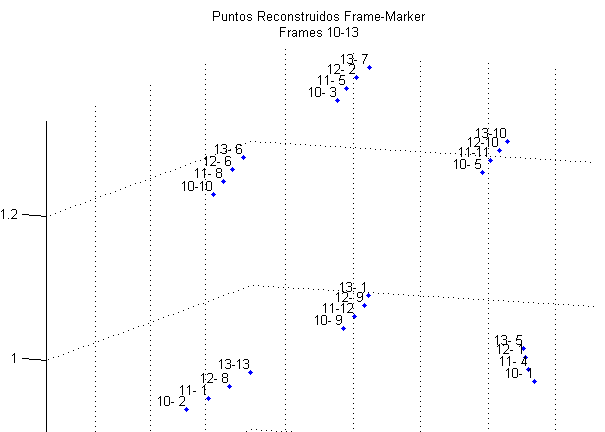
\includegraphics[scale=0.8]{img/Tracking/00_Salida_Reconstruccion}
\end{center}
\caption{Resultado de aplicar un umbral de valor 200.}
\label{reconstr_00}
\end{figure}

\subsection{Implementación}



\subsubsection{Enlazado en régimen}



\subsubsection{Enlazado inicial y final}



\subsubsection{Inventario de trayectorias}



\subsection{Resultado y Analisis}


